\section{COAXIAL RF LINE}
\subsection{Task description}
The objective of this task is to measure the standing wave ratio and the reflection coefficient of different loads connected to a coaxial transmission line using a signal analyzer\cite{CXA_SA}, the loads to be used are: 

\begin{itemize}
	\setlength{\itemsep}{0pt}
	\setlength{\parskip}{0pt}
	\item Open
	\item Short
	\item 50$\Omega$
	\item 100$\Omega$
	\item 25$\Omega$
	\item Capacitive load
\end{itemize}

The transmission line is fed with a sine wave signal of +10dBm at 310 MHz from an RF signal generator\cite{RF_SG}.
\subsection{Schematic}
Figure~\ref{fig:5} shows the measurement configuration of the coaxial transmission line and a movable E-field probe.
\begin{figure}[ht!]
    \centering
    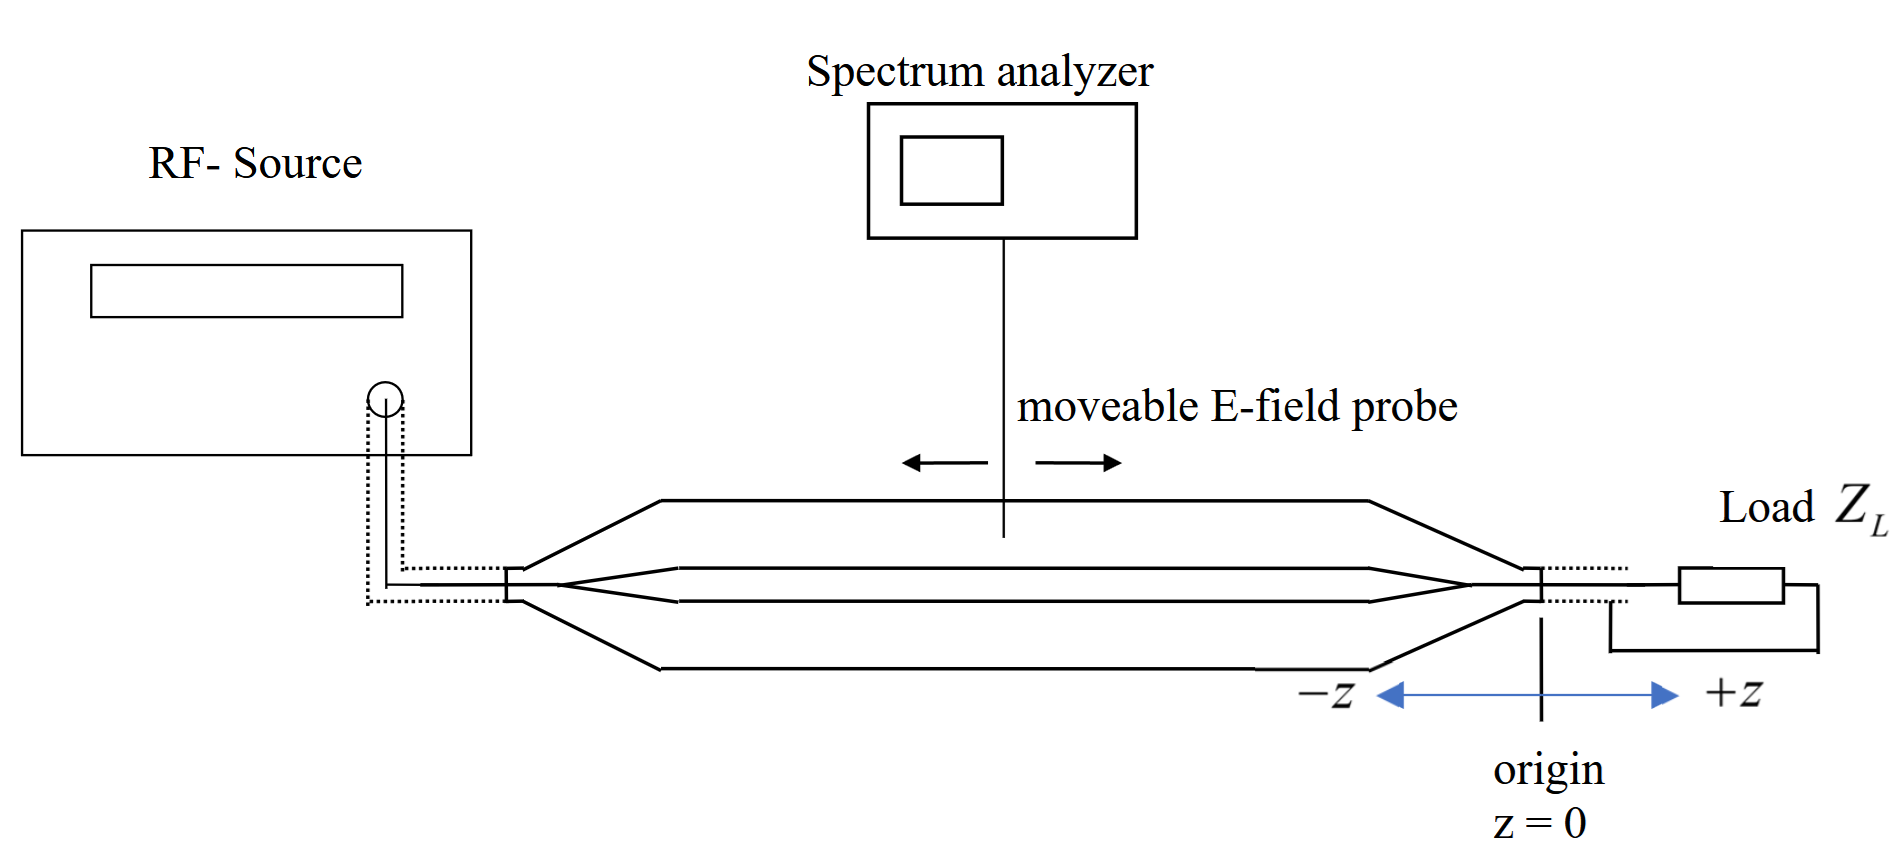
\includegraphics[page=1,width=0.8\linewidth]{src/diagrams/RF_1/Schematic_1.png}
    \caption{\centering Schematic of the measurement setup used, with RF coaxial line, E-field probe and the load.}
    \label{fig:5}
\end{figure}
\\
The schematic above shows the four main components used in this measurement setup. These are:
\begin{itemize}
	\setlength{\itemsep}{0pt}
	\setlength{\parskip}{0pt}
	\item The RF signal generator\cite{RF_SG}, which provides the excitation signal.
	\item The spectrum analyzer\cite{CXA_SA} with a movable E-field probe.
	\item The coaxial transmission line which is traced by the probe.
	\item The load at the end of the line; this can be replaced by any of the six terminations described earlier.
\end{itemize}

\newpage
\subsection{Formulas and calculations}
\subsubsection{\textbf{Calculation of the wave velocity:}}
The following formula \ref{eq:1_CO} is used to calculate the wave velocity$v$. \\
\begin{gather}
	v = f \cdot \lambda 							\label{eq:1_CO}
\end{gather}
$f$ (frequency) = 310MHz\\
$\lambda$ (wavelength) = $2 \cdot \Delta d $\\

The term $\Delta d$ is given by the difference between the points of two adjacent minima. \\For the different loads, this value (obtained from correlating the chart \ref{fig:chart1}, and the tables \ref{tab:power_plots_1} \& \ref{tab:power_plots_2}) is:
\begin{itemize}
	\setlength{\itemsep}{0pt}
	\setlength{\parskip}{0pt}
	\item Open: 48.3cm
	\item Short: 48.2cm
	\item Capacitive load: 48.5cm
\end{itemize} 

Averaging these values to minimize tiny individual measurement errors, obtained $\Delta d$ = 48.33cm.\\

Inferred wavelength: This measured value for wavelength is obtained using the formula \ref{eq:4_CO} : 
\begin{gather}
	\lambda = 2 \cdot \Delta d 						\label{eq:4_CO} \\
	\lambda = 96.667cm
\end{gather}

Hence, \\
Wave velocity (in m/s) is:
\begin{gather}
	v = 310 \times 10^6 \cdot 0.96451 				\nonumber \\
	v = 2.9966 \times 10^8							\label{eq:3_CO}
\end{gather}

\subsubsection{\textbf{Calculation of the Voltage Standing Wave Ratio (VSWR) and reflection coefficient metrics:}}

Equation~\ref{eq:vswr_voltage} gives the definition of VSWR. Since the spectrum analyzer provides power values, VSWR can also be expressed in terms of the measured power ratio:
\begin{gather}
	\mathrm{VSWR} = \frac{V_{\max}}{V_{\min}} \label{eq:vswr_voltage} \\
	\mathrm{VSWR} = \sqrt{\frac{P_{\max}}{P_{\min}}} \nonumber
\end{gather}

Since $P_{\max}$ and $P_{\min}$ must be in linear units, the measured values in dBm are converted using:
\begin{gather}
	\frac{P_{\max}}{P_{\min}} = 10^{\frac{P_{\max,\mathrm{dBm}} - P_{\min,\mathrm{dBm}}}{10}} \nonumber
\end{gather}

Finally, VSWR for each termination is calculated as:
\begin{gather}
	\mathrm{VSWR} = 10^{\frac{P_{\max,\mathrm{dBm}} - P_{\min,\mathrm{dBm}}}{20}} \label{eq:vswr_power}
\end{gather}

Using values from tables~\ref{tab:power_plots_1} and~\ref{tab:power_plots_2}, the calculation of VSWR, and subsequently the magnitude of it's reflection coefficient (using the relation~\ref{eq:rho_mag}), is made possible:
\begin{gather}
	|\mathrm{\underline{\rho_0}}| = \frac{\mathrm{VSWR}-1}{\mathrm{VSWR}+1} \label{eq:rho_mag} \\
	\angle \rho = \text{from the position of the minima on the line} \label{eq:rho_phase}
\end{gather}

\subitem{\textbf{VSWR for Open load:}}
\begin{gather}
	\mathrm{VSWR} = 10^{\frac{-17.0 - (-73.0)}{20}}
	= 10^{\frac{56.0}{20}}
	= 10^{2.8}
	\approx 630.96 \label{eq:vswr_open}\\
	|\rho| = \frac{629.96}{631.96}
	\approx 0.997 \label{eq:mag_open}
\end{gather}

\subitem{\textbf{VSWR for Short:}}
\begin{gather}
	\mathrm{VSWR} = 10^{\frac{-18.7 - (-64.0)}{20}}
	= 10^{\frac{45.3}{20}}
	= 10^{2.265}
	\approx 184.29 \label{eq:vswr_short} \\
	|\rho| = \frac{183.29}{185.29}
	\approx 0.989 \label{eq:mag_short}
\end{gather}

\subitem{\textbf{VSWR for 100$\Omega$ load:}}
\begin{gather}
	\mathrm{VSWR} = 10^{\frac{-20.8 - (-27.3)}{20}}
	= 10^{\frac{6.5}{20}}
	= 10^{0.325}
	\approx 2.11 \label{eq:vswr_100} \\
	|\rho| = \frac{1.11}{3.11}
	\approx 0.357 \label{eq:mag_100}
\end{gather}

\subitem{\textbf{VSWR for 25$\Omega$ load:}}
\begin{gather}
	\mathrm{VSWR} = 10^{\frac{-18.0 - (-28.7)}{20}}
	= 10^{\frac{10.7}{20}}
	= 10^{0.535}
	\approx 3.43 \label{eq:vswr_25} \\
	|\rho| = \frac{2.43}{4.43}
	\approx 0.549 \label{eq:mag_25}
\end{gather}

\subitem{\textbf{VSWR for 50$\Omega$ load:}}
\begin{gather}
	\mathrm{VSWR} = 10^{\frac{-22.9 - (-24.0)}{20}}
	= 10^{\frac{1.1}{20}}
	= 10^{0.055}
	\approx 1.13 \label{eq:vswr_50} \\
	|\rho| = \frac{0.13}{2.13}
	\approx 0.061 \label{eq:mag_50}
\end{gather}

\subitem{\textbf{VSWR for Capacitive load:}}
\begin{gather}
	\mathrm{VSWR} = 10^{\frac{-18.3 - (-53.8)}{20}}
	= 10^{\frac{35.5}{20}}
	= 10^{1.775}
	\approx 59.57 \label{eq:vswr_cap} \\
	|\rho| = \frac{58.57}{60.57}
	\approx 0.967 \label{eq:mag_cap}
\end{gather}

\subsection{Table with measurement results}
Tables~\ref{tab:power_plots_1} and~\ref{tab:power_plots_2} (placed in the appendix section of this document) present the measured power values at different positions along the coaxial RF line for different terminations.

\newpage
\subsection{Simulation curves and diagrams} 
Figures~\ref{fig:screen1} shows the spectrum analyzer output after making basic settings such as center, span, magnitude, sweep time, and residual bandwidth.
\begin{figure}[ht!]
	\centering
	\includegraphics[page=4,width=0.7\linewidth]{src/diagrams/RF_1/Screen1}
	\caption{\centering Spectrum analyzer output on proper setting of required parameters.}
	\label{fig:screen1}
\end{figure}

Illustrated in Figure~\ref{fig:chart1} is the measured location-dependent signal power values obtained along the coaxial transmission line with the RF Spectrum Analyzer for termination loads: Open, Short and 100$\Omega$ loads. \\The measurements were taken over a range of 35.0cm to 167.0cm, measured from the termination load.
\begin{figure}[ht!]
    \centering
    \includegraphics[page=4,width=0.85\linewidth]{src/diagrams/RF_1/Chart_1}
    \caption{\centering Measured power values for open, short and 100$\Omega$ terminations.}
    \label{fig:chart1}
\end{figure}
\\Similar to \ref{fig:chart1}, illustrated in Figure~\ref{fig:chart2} is the measured location-dependent signal power values obtained along the coaxial transmission line with the RF Spectrum Analyzer for termination loads: 25$\Omega$, 50$\Omega$ and purely capacitive loads.
\begin{figure}[ht!]
	\centering
	\includegraphics[page=4,width=0.85\linewidth]{src/diagrams/RF_1/Chart_2}
	\caption{\centering Measured power values for 25$\Omega$, 50$\Omega$ and capacitive load terminations.}
	\label{fig:chart2}
\end{figure}
\\A consolidated figure with all 6 measurements curves on the same chart is present in the appendix Figure~\ref{fig:chart3}
\FloatBarrier
\subsection{Discussion} 
\begin{itemize}
  \item \textbf{Noise analysis of a single stage emitter circuit}:\\
  Noise analysis of the single stage emitter circuit (figure~\ref{fig:6}) reveals that $R_g$ contributes most to the total noise (brown trace).
  \item \textbf{OpAmp noise model check}:\\
  A simple voltage follower circuit was built with LM4562 and using cursors, the simulated noise density $e_n$ was read at 10\,Hz as well as 1.0\,kHz and compared to the datasheet values (see table~\ref{tab:sim_2}).
  \item \textbf{Noise analysis of inverting and non-inverting amplifier circuits}:\\
  The simulated output noise spectral density for these circuits with gain-10 amplifiers is shown in (figures~\ref{fig:8} and~\ref{fig:112}). The spectrum shows the expected behaviour: increased low-frequency noise due to flicker noise and an approximately flat mid-band (white) noise floor. The change in slope marks the 1/f corner frequency.
\end{itemize}
